% ***********************************************************************************
% Pure LaTeX part to be inserted in a document (be careful of depencies of packages & commands)
% Prepared by XXX and YYY under the supervision of Arnaud de La Fortelle
% Fall 2017
% 2D heat diffusion subsection of the modeling part
% ***********************************************************************************

\subgroup{2}{Qingan Zhao and Ruitong Zhu}

\paragraph{Description}
The aim of this part is to describe and model a PDE that describes temperature dynamics in a two-dimensional body via heat conduction.
Basically, heat conduction is the exchange of heat from regions of higher temperatures into regions with lower temperatures, which varies in the transfer rate for different materials.
%\\\\
%COMMENT: almost never put yourself editing commands. Otherwise use LaTeX commands like \bigskip

Consider a thin flat body with a constant thickness $h$ and uniform density $\rho'$. Assume that the faces of the thin body are in perfect insulation, which means there is no heat flow travel in the out-of-plane direction of the body. Hence, heat can only flow in the direction within the plane of the body, which turns into a two-dimensional problem. Then a two-dimensional coordinate system is established such that each point of the body can be described with a coordinate $(x,y)$. Then the (2D-uniform) density of the body is $\rho = \rho' h$. Denote the temperature function of each point by $T$ so that the temperature of the body at position $(x,y)$ and time $t$ are described as $T(x,y,t)$, as shown in Figure~\ref{heatSystem.fig}. The goal is to derive $T(x,y,t)$ when there is no internal heat source.
%COMMENT: introduce your notation quickly. Best to be intuitive: T is more intuitive for temperature than u

\begin{figure}[htb]
	\centering
	\includegraphics[width=10cm]{heatSystem.pdf}       
	\caption{System description in 2 dimensions}\label{heatSystem.fig}
%COMMENT: do not count yourself: TODO use intensively \label and \ref
\end{figure}

\paragraph{Model}
Consider a small rectangular element of the body with vertices $(x,y)$, $(x+\ud x,y)$, $(x, y+\ud y)$, and $(x+\ud x, y+\ud y)$. The heat flows are shown in Figure~\ref{heatElement.fig}.
\begin{figure}[htb]
	\centering
	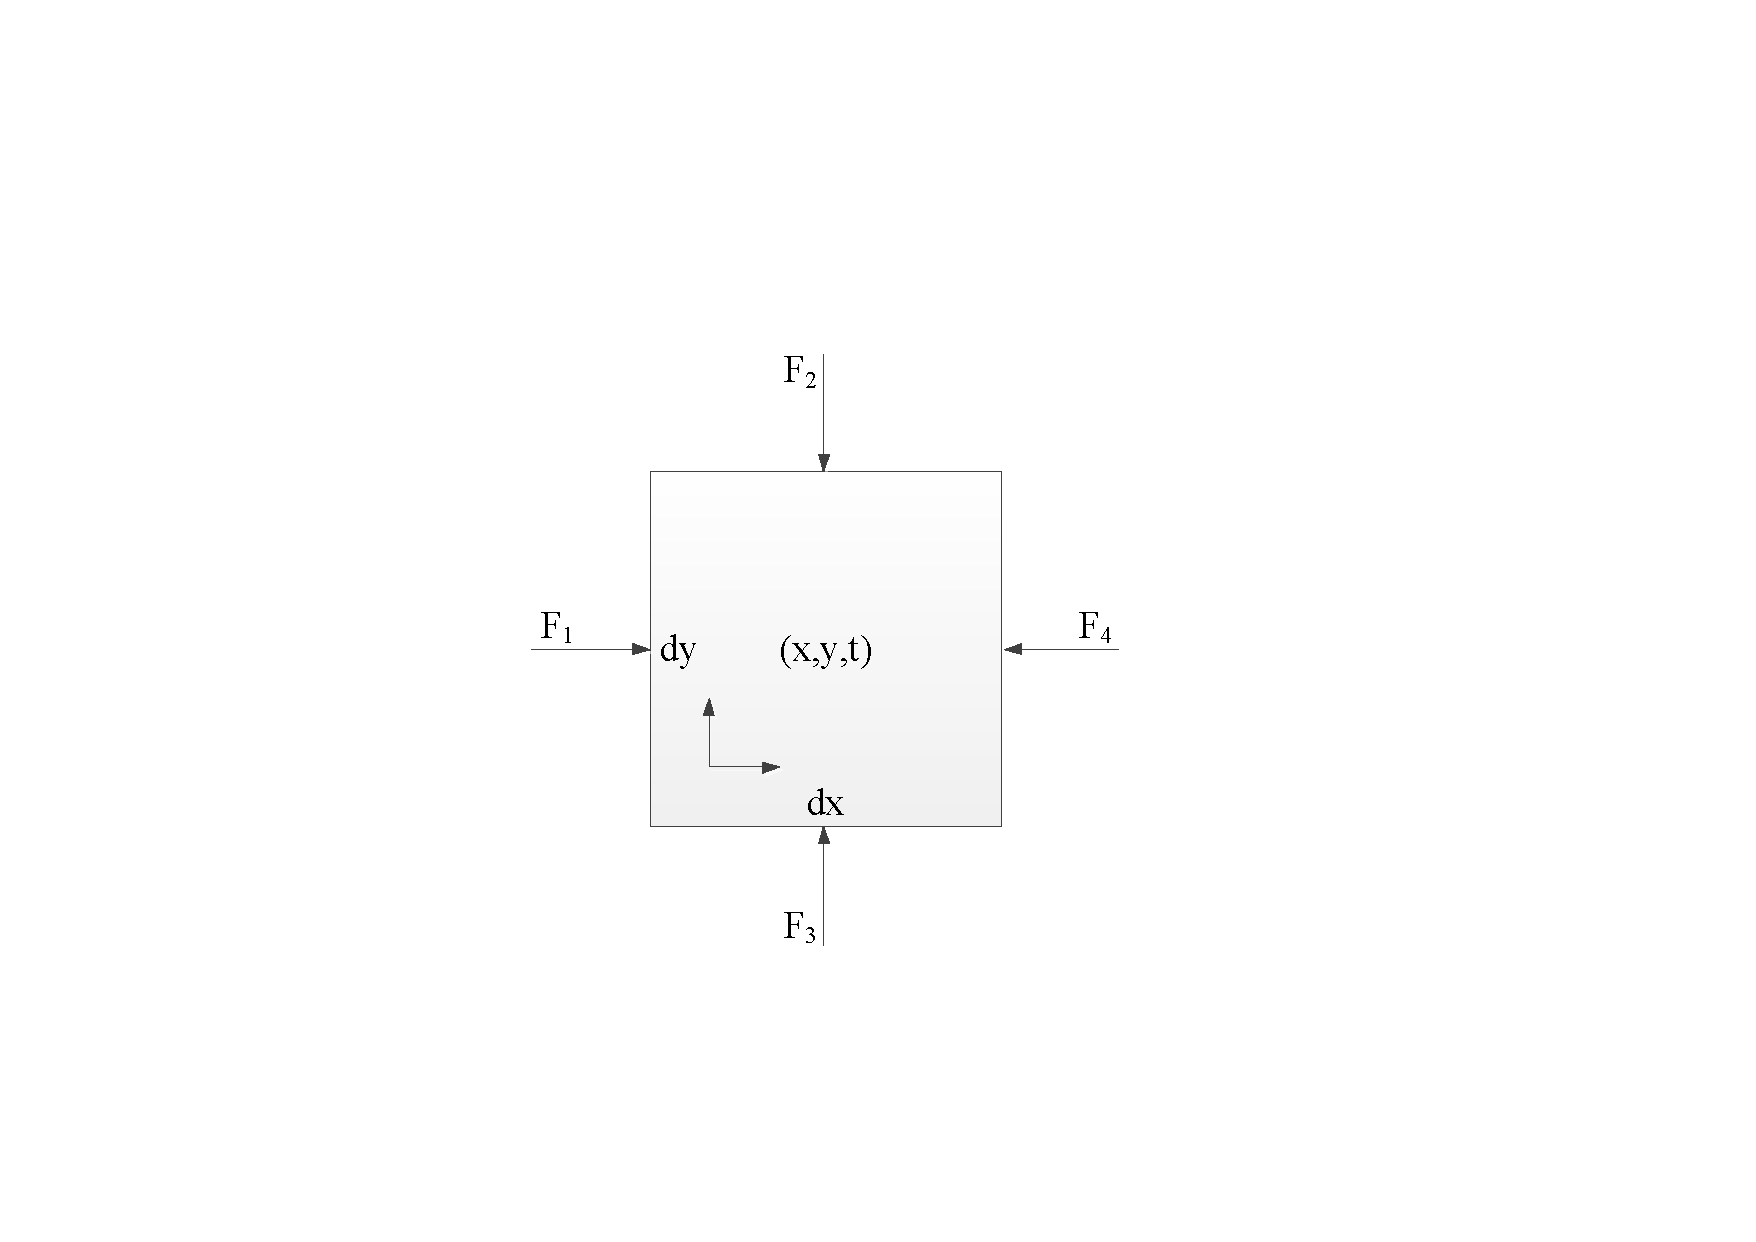
\includegraphics[width=8cm]{heatElement.pdf}       
	\caption{Heat flows in a small rectangular element of the body}\label{heatElement.fig}
\end{figure}

\noindent The heat amount $Q$ (i.e the thermal energy) of the rectangular element at time $t$ is: 
\begin{equation}
Q(x,y,t)=C m T(x,y,t)
\end{equation}
where $C$ is called \emph{heat capacity}, which is a supposed to be constant (assuming the material is uniform and temperature do not vary too much); $m = \rho A$ is the mass of the rectangular element where $A$ its surface.
The rate of thermal energy change with respect to time is therefore:
\begin{equation}\label{thermalEnergyChange.eq}
\frac{\partial Q}{\partial t} = C\rho \ud x \ud y\frac{\partial T}{\partial t}
\end{equation}
As shown in Figure~\ref{heatElement.fig}, the incoming flow is $F_1 + F_2 + F_3 + F_4$. Denote the heat flux $\vec q$ in horizontal and vertical directions by $q_x$ and $q_y$, then we have:
\begin{eqnarray} %COMMENT: the best environment for multiple equation; you can align with & as shown below TODO replace by eqnarray
F_1 &=& q_x(x,y,t)\ud y\label{flow1}\\
F_2 &=& -q_y(x,y+\ud y,t)\ud x\label{flow2}\\
F_3 &=& q_y(x,y,t)\ud x\label{flow3}\\
F_4 &=& -q_x(x+\ud x,y,t)\ud y\label{flow4}
\end{eqnarray}
%Sum up $F_1\sim F_4$:
%COMMENT: not very explicit, better this way:
Now, we know that according to energy conservation, the thermal energy variation of any small element (as in Equation~(\ref{thermalEnergyChange.eq})) is equal to the total incoming heat flow.  By putting the partial flows as in Equations~(\ref{flow1})-(\ref{flow4}), this conservation principle yields:
\begin{equation}\label{thermalEnergyChange.eq2}
C\rho \ud x \ud y\frac{\partial T}{\partial t} = \ud y [q_x(x,y,t)-q_x(x+\ud x,y,t)]+\ud xh[q_y(x,y,t)-q_y(x,y+\ud y,t)]
\end{equation}
%COMMENT: use \emph to emphasize
Now, another physical principle, \emph{Fourier's Law}, states that the heat flow is (negatively) proportional to the gradient of temperature:
\begin{equation}\label{FourierLaw.eq}
\vec q = -k\nabla T
\end{equation}
where $k$ is known as the thermal conductivity of the material (also considered as a constant). Then $q_x$ and $q_y$ are expressed as:
\begin{equation}
\begin{split}
q_x=-k\frac{\partial u}{\partial x}\\
q_y=-k\frac{\partial u}{\partial y}
\end{split}
\end{equation}
%TODO: replace numbers by \ref (with the appropriate \label
Hence, Equation (4) can be written as:
\begin{equation}
\frac{\partial Q}{\partial t}=k\ud yh\left(\frac{\partial u(x+\ud x,y,t)}{\partial x}-\frac{\partial u(x,y,t)}{\partial x}\right)+k\ud xh\left(\frac{\partial u(x,y+\ud y,t)}{\partial y}-\frac{\partial u(x,y,t)}{\partial y}\right)
\end{equation}
Combine Equation (2)(7):
\begin{equation}
\frac{\partial u(x,y,t)}{\partial t}=\frac{k}{c\rho}\left(\frac{\partial ^2 u(x,y,t)}{\partial x^2}+\frac{\partial ^2 u(x,y,t)}{\partial y^2}\right)
\end{equation}
Denote $k/c\rho$ by $a^2$, and the two-dimensional heat equation can be drawn:
\begin{equation}
\frac{\partial u}{\partial t}=a^2\left(\frac{\partial ^2 u}{\partial x^2}+\frac{\partial ^2 u}{\partial y^2}\right)
\end{equation}
%COMMENT: look at the use of \left( and \right) to have nice parentheses
We also need to specify initial conditions and boundary conditions in order to solve the equation. For initial conditions, we assume that in domain $\Omega$:
\begin{equation}
T(x,y,0)=\phi(x,y) 
\end{equation}
As for boundary conditions, it could be devided into two different situations according to the domain $\Omega$. If $\Omega=R^2$, we don't have to worry about the boundary, which means the equation can be solved soly based on the initial condition defined on $R^2$. But if there is a boudary $\partial\Omega$, in this case, the boundary conditions can be described as: 
\begin{equation}
T(x,y,t)|_{(x,y)\in\partial\Omega} =g(x,y,t) 
\end{equation}
